\chapter{Forest for the Trees}
\lettrine[lines=4]{T}{rees} are another special kind of graph which we did not discuss in the previous chapter. Trees are somewhat unique compared to the other types of specialty graphs described before as they allow us certain algorithms to perform to solve different problems. Before we go in depth into trees, we must first define an operation and some other terms.

\section{Definitions}
Let $G_1$ and $G_2$ be graphs. Then $G_1 \cup G_2$ is the \textbf{union} of $G_1$ and $G_2$ with the vertex set $V = V(G_1) \cup V(G_2)$ and edge set $E = E(G_1) \cup E(G_2)$. Now, let's establish some more definitions:
\begin{description}
    \item[Disconnected:] A graph is \textbf{disconnected} if it is the union of two graphs. Here is an example of a disconnected graph:
    \begin{center}
        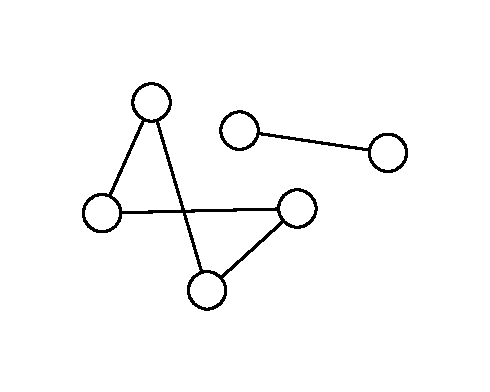
\includegraphics[width=0.3\textwidth]{Chapter2/disconnect.pdf}
    \end{center}
    \item[Connected:] A graph is \textbf{connected} if it is not disconnected (wow). Here is an example of a connected graph:
    \begin{center}
        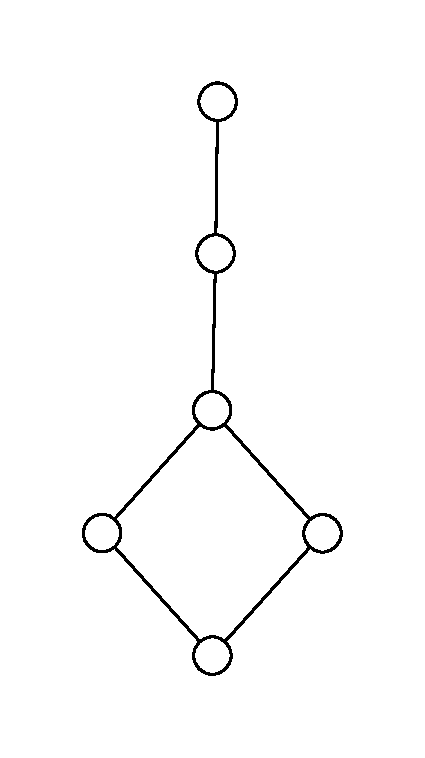
\includegraphics[width=0.3\textwidth]{Chapter2/connect.pdf}
    \end{center}
    \item[Component:] A \textbf{component} graph is one graph which makes up part of a union. In $G = G_1 \cup G_2$, $G_1$ and $G_2$ are components.
\end{description}

We can also define the \textbf{subtraction} of a set of edges $F$ from a graph $G$. We say that $G - F$ is the graph resulting in the removal of the edges in $F$ from $G$. Suppose we have the following graph $G$:
\begin{center}
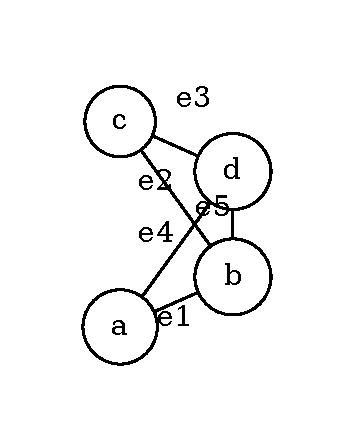
\includegraphics[width=0.3\textwidth]{Chapter2/sub0.pdf}
\end{center}
Then the following are different subtractions from $G$.
\begin{figure}[h]
    \subfloat[$G - \{e1\}$]{
        \begin{minipage}[c][1\width]{0.3\textwidth}
            \centering
            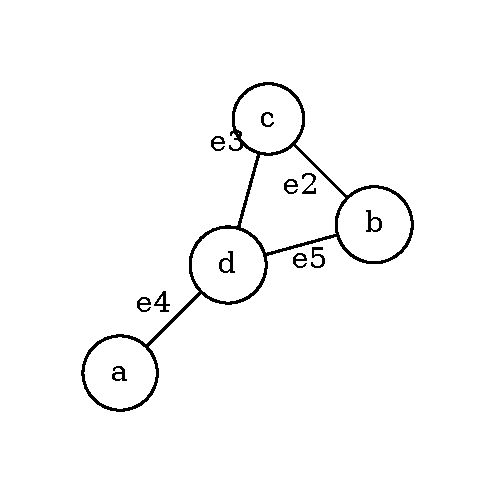
\includegraphics[width=1.\textwidth]{Chapter2/sub1.pdf}
        \end{minipage}
    }
    \subfloat[$G - \{e2\}$]{
        \begin{minipage}[c][1\width]{0.3\textwidth}
            \centering
            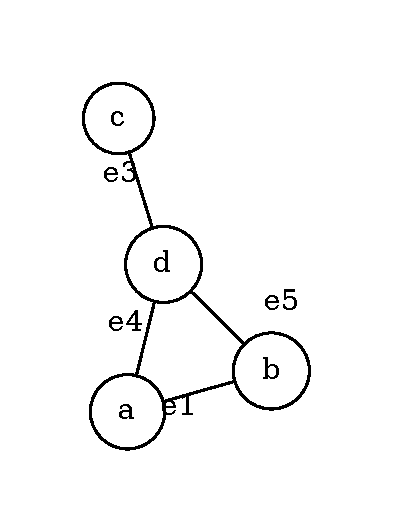
\includegraphics[width=\textwidth]{Chapter2/sub2.pdf}
        \end{minipage}
    }
    \subfloat[$G - \{e1, e2\}$]{
        \begin{minipage}[c][1\width]{0.3\textwidth}
            \centering
            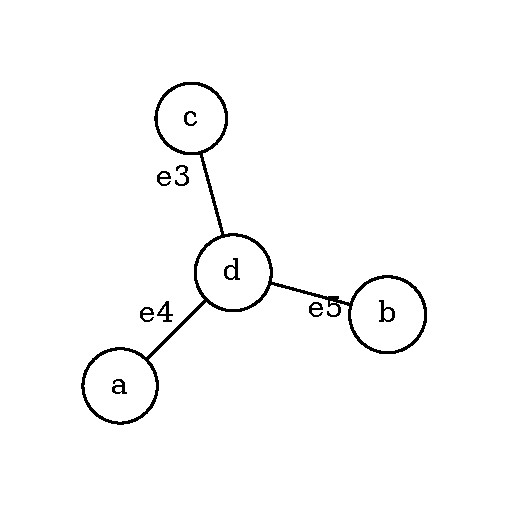
\includegraphics[width=\textwidth]{Chapter2/sub12.pdf}
        \end{minipage}
    }
\end{figure} 

Let's define a new type of graph. A connected graph that is regular of degree 2 is called a \textbf{cycle}, which we denote $C_n$. Here is an example of a cycle, $C_5$:
\begin{center}
    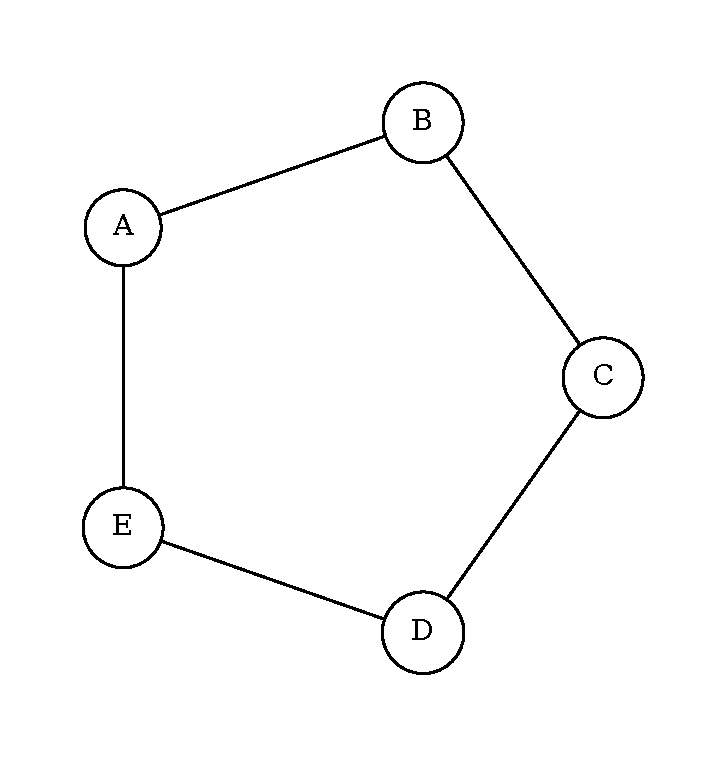
\includegraphics[width=0.3\textwidth]{Chapter2/c5.pdf}
\end{center}

A useful operation on graphs is to take the complement. The \textbf{complement} of a graph $G$ is the graph $\overline{G}$, with vertex set $V(\overline{G}) = V(G)$, with two vertices adjacent in $\overline{G}$ if and only if they are \emph{not} adjacent in $G$. Given $C_5$, we can fine its complement, $\overline{C_5}$:
\begin{center}
    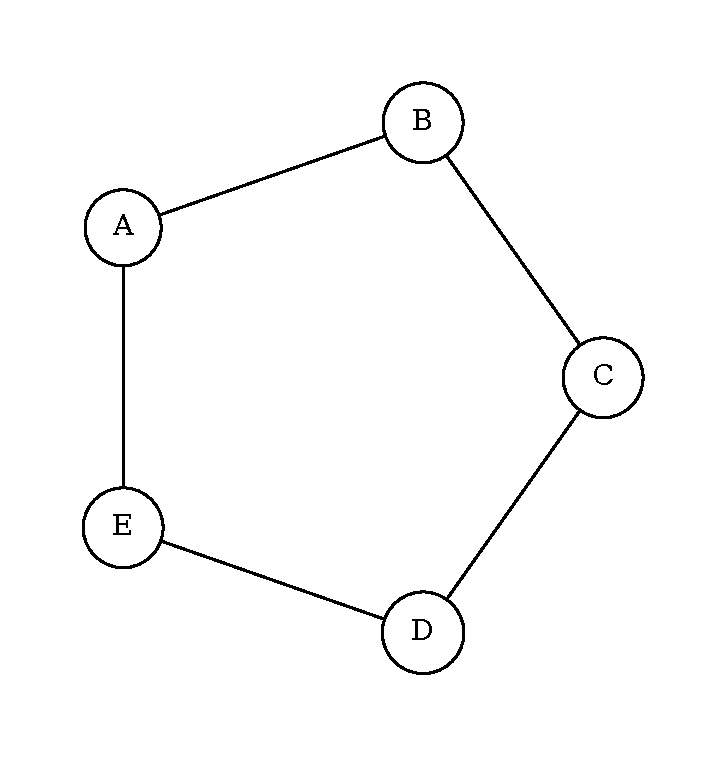
\includegraphics[width=0.3\textwidth]{Chapter2/c5.pdf}
    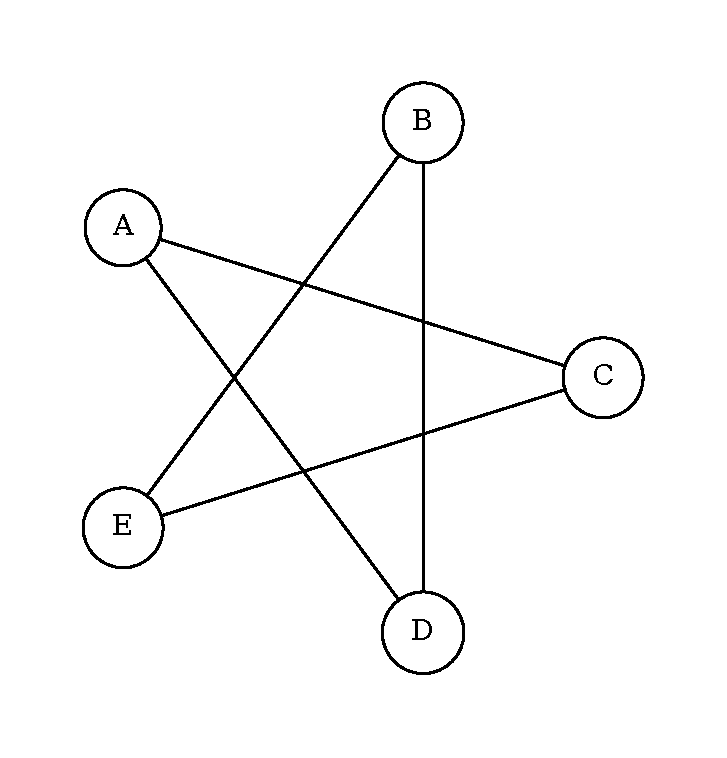
\includegraphics[width=0.3\textwidth]{Chapter2/c5comp.pdf}
\end{center}
In this particular example, notice that $C_5 \sim \overline{C_5}$, so $C_5$ is what we call \textbf{self-complementary} - it is isomorphic to its own complement.

\section{Trailblazing}
We've defined what graphs are as a construct, but how do we actually navigate from one point to another? There are different ways to navigate from vertex to vertex, and each form of navigation takes on different attributes. Consider the following graph $G_0$:
\begin{center}
    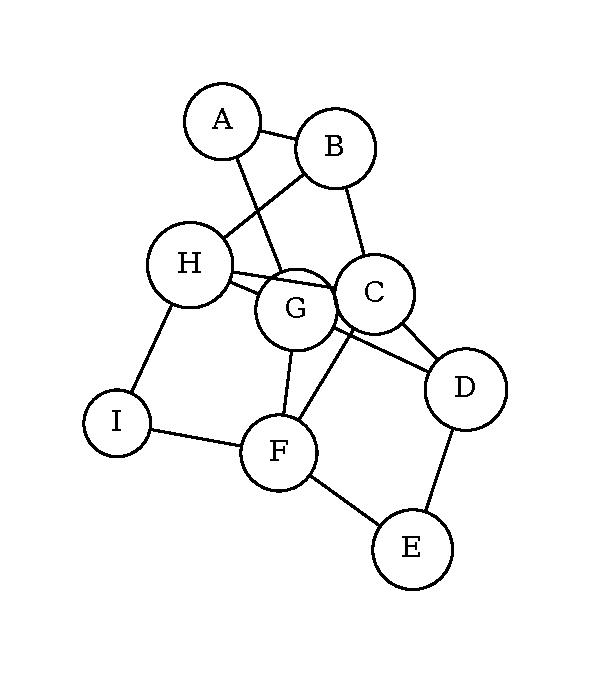
\includegraphics[width=0.5\textwidth]{Chapter2/nav.pdf}
\end{center}
Let's define some of the different ways we can navigate through $G_0$:
\begin{description}
    \item[Walk:] A \textbf{walk} in a graph $G$ is any finite sequence of edges, $v_0v_1, v_1v_2, v_2v_3, \ldots, v_{k-1}v_k$. The initial vertex is denoted $v_0$, and the final vertex is denoted $v_k$. The \textbf{length} of the walk is $k$. Here is an example of a walk in $G_0$:
    \begin{center}
        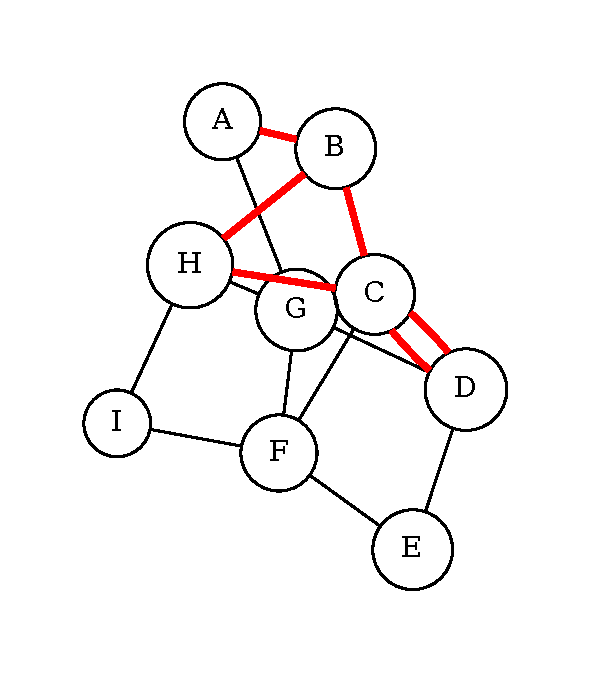
\includegraphics[width=0.5\textwidth]{Chapter2/walk.pdf}
    \end{center}
    Here, the walk shown begins at node $A$. The walk is $AB, BH, HC, CD, DC$, $CB$. The length of this walk is 6.
    \item[Trail:] A walk where all the \emph{edges} are distinct is a \textbf{trail}. The walk observed above is not a trail, since the edge $\{C, D\}$ is repeated. Thus, a variation of this as a trail might be:
    \begin{center}
        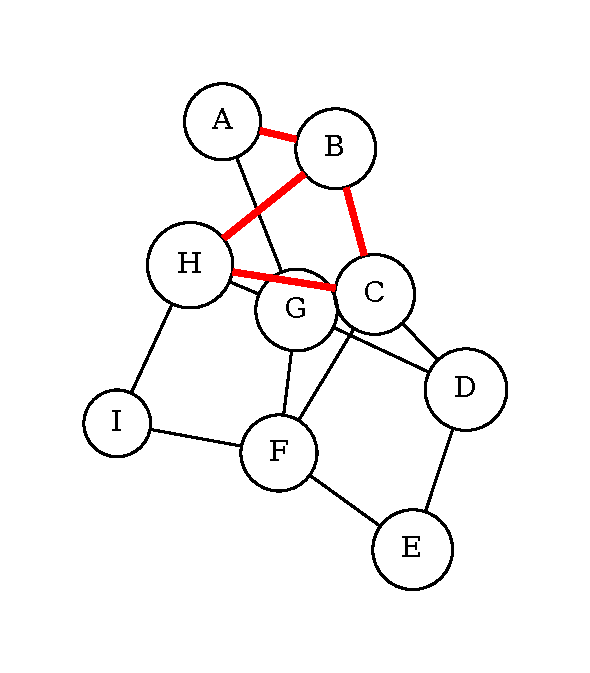
\includegraphics[width=0.5\textwidth]{Chapter2/trail.pdf}
    \end{center}
    The trail here is $AB, BH, HC, CB$.
    \item[Path:] A trail where all the \emph{vertices} are unique is called a \textbf{path}. The trail above would not be a path, as the vertex $B$ is visited twice. Here is an example of a path in $G_0$:
    \begin{center}
        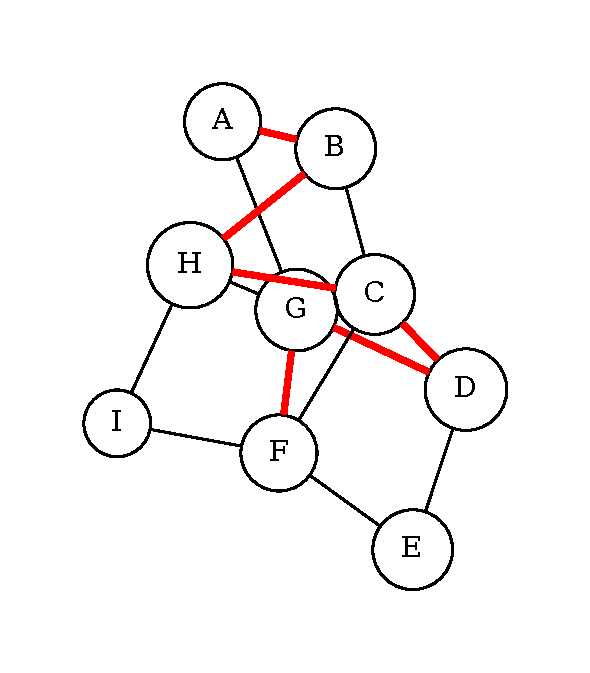
\includegraphics[width=0.5\textwidth]{Chapter2/path.pdf}
    \end{center}
    This path is $AB, BH, HC, CD, DG, GF$.
    \item[Cycle:] A \textbf{closed} path (where $v_0 = v_k$) has at least one edge, then it is a \textbf{cycle}. Here is an example of a cycle in $G_0$:
    \begin{center}
        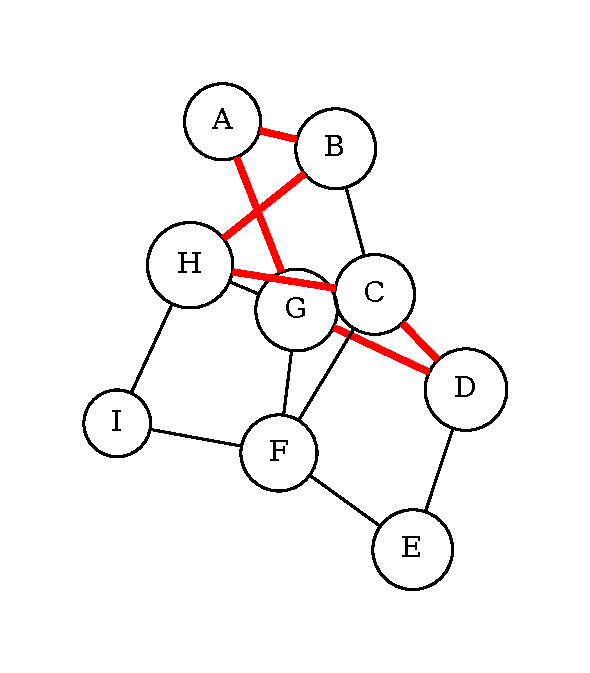
\includegraphics[width=0.5\textwidth]{Chapter2/cycle.pdf}
    \end{center}
    This cycle is $AB, BH, HC, CD, DG, GA$.     
\end{description}
\section{The Lorax}
We have the terminology we need to finally describe the subjects of this chapter: trees and forests. 
\begin{description}
    \item[Forest:] A \textbf{forest} is a graph with no cycles. It need not necessarily be connected, so long as there are no cycles. Here is an example of a forest:
    \begin{center}
        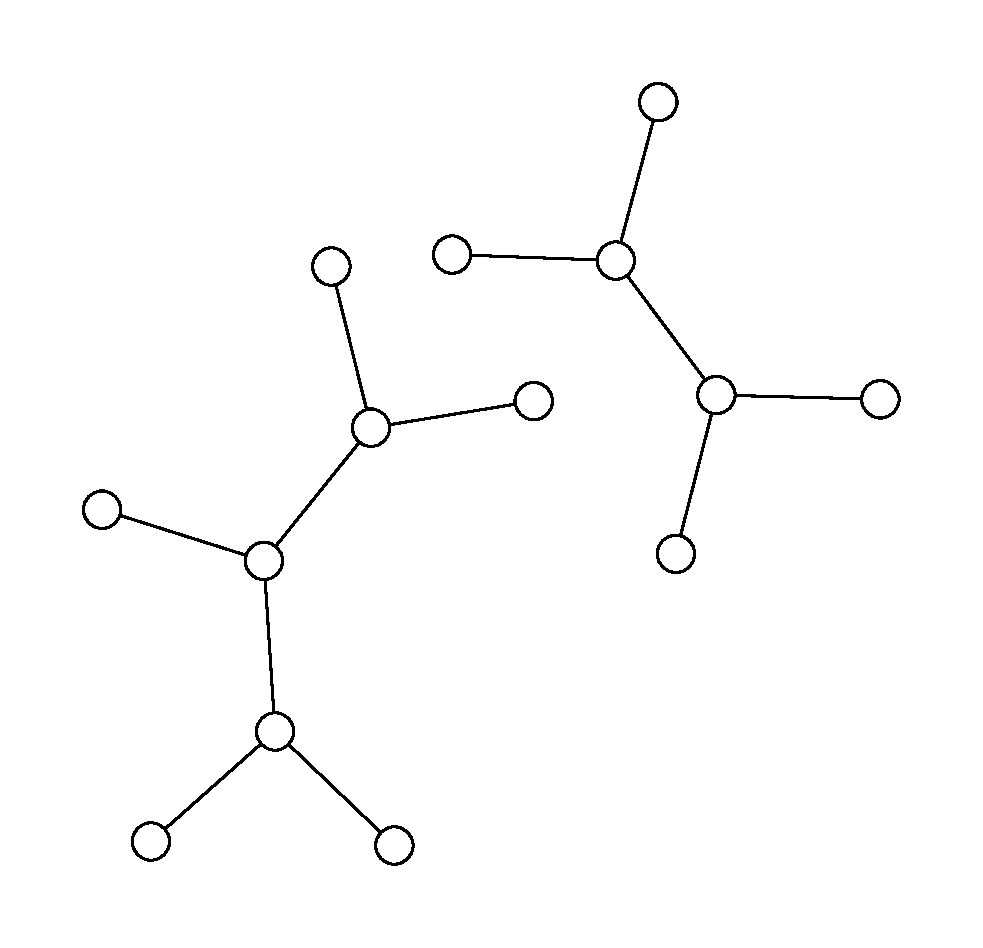
\includegraphics[width=0.5\textwidth]{Chapter2/forest.pdf}
    \end{center} 
    \item[Tree:] A \textbf{tree} is a connected forest. Here is an example of a tree:
    \begin{center}
        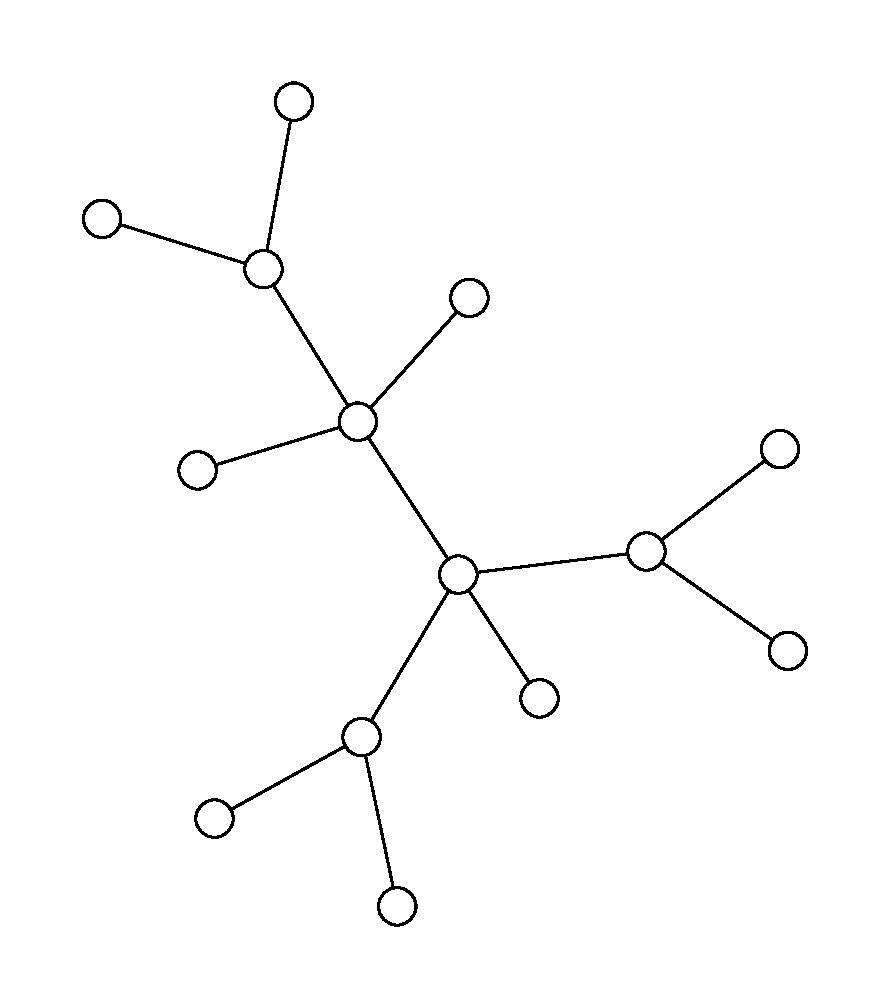
\includegraphics[width=0.5\textwidth]{Chapter2/tree.pdf}
    \end{center} 
\end{description}
Trees come in many different shapes and sizes, the count of which grows quickly as more nodes are introduces. For example, there is only one tree of one, two, and three nodes. Once we introduce a fourth node, we see that there are two distinct trees of four nodes. The more nodes we introduce, the more rapidly the count of distinct isomorphisms increases. 

\section{(Minimum) Spanning Trees}
While fundamentally trees and forests are just different kinds of graphs, they are useful tools when used in conjunction with graphs. One example of this is the \textbf{spanning tree} of a graph. The spanning tree of a graph $G$ is a tree which includes all vertices of the graph $G$. Another way to imagine this is a non-cyclic representation of $G$. On top of spanning trees, we have \textbf{minimum spanning trees} (MSTs). The MST of a graph $G$ is a spanning tree whose whose total weight is minimal compared to all spanning trees. First, let's define what a weight is.

A \textbf{weight} is a numerical value assigned to an edge. This number is representative of the total cost of traversing from one vertex to another along that particular edge - some edges may be cheaper, others may be longer. We assume that these weights are strictly non-negative (so for a weight $n, n \in \mathbb{Z}^*$). The total weight of a graph is the sum of the weights of all edges.

Again, the MST for a graph $G$ is a spanning tree with minimal weight. How do we find the minimum spanning tree for a graph? There are three popular algorithms which solve this problem: Prim's Algorithm, Kruskal's Algorithm, and Bor\r{u}vka's Algorithm.
\subsection{Prim's Algorithm}
Prim's Algorithm was originally developed by Czech mathematician Vojt\v{e}ch Jarn\'{i}k in 1930, but was later published by Robert Prim and Edsger Dijkstra in 1959\cite{PrimsAlgo}. Prim's algorithm focuses on the vertices of a graph, and considers edges incident to the vertices in the MST as it grows. Below is a quick pseudocode representation of this algorithm\cite{IntroToAlgo}.

\begin{algorithm}
    \DontPrintSemicolon
    \caption{Prim's Algorithm}

    \KwData{Weighted graph $G$, root vertex $v_0$}
    \KwResult{Minimum spanning tree $T$}
    \SetKwFunction{setw}{Weight}
    \SetKwFunction{setp}{Parent}
    \SetKwFunction{exmin}{GetMinVertex}
    \SetKwFunction{edge}{EdgeWeight}
    \SetKwFunction{adj}{AdjacentTo}

    \For{$v \in V(G)$}{
        \setw{v} $\gets \infty$\;
        \setp{v} $\gets$ null\;
    }
    \setw{$v_0$} $\gets 0$\;
    $Q \gets V(G)$\;
    \While{$Q \neq \emptyset$}{
        $u \gets$ \exmin{$Q$}\;
        \ForEach{$v \in$ \adj$(u)$}{
            \If{$v \in Q$ and \edge{$u, v$} $<$ \setw{$v$}}{
                \setp{$v$} $\gets u$\;
                \setw{$v$} $\gets$ \edge{$u, v$}
            }
        }
    }
\end{algorithm}

Given a root node $v_0$ to begin the construction of the MST, the objective for the algorithm is to construct a tree based on weights from nodes already examined. The preliminaries of this algorithm look very much like Dijkstra's algorithm (discussed later), where we initialize the weights of all vertices to infinity, and the root node to zero. Additionally, we want to keep track of the edge through which we reach the vertex, so we initialize the parent to null. 

We use $Q$ as a minimum heap structure to grab the smallest weighted vertex, calling it $u$. The idea is to examine all adjacent vertices to $u$, and update their current weight if following the edge from $u$ to said vertex is better than what was found previously. If so, we set the parent of that vertex to $u$, and update the weight. 

Once $Q$ is exhausted, we will have determined the minimal edges connecting each vertex in the graph, resulting in the MST. This formalization of the algorithm is a bit dense, so the simplified version of what was discussed in class is as follows:

First, grab a vertex $v$ at random from a graph $G$, and initialize a tree $T$ as empty, and a set $P$ with $v$. $P$ will be our set of visited vertices, and $T$ will be the collection of edges which make the MST. Find the minimum weighted edge connecting a vertex in $P$ to a vertex not in $P$, and add this edge to $T$ and the vertex to $P$. Repeat until $P = V(G)$. The collection of edges $T$ will be the MST.

This algorithm is greedy - at each decision point, we follow the smallest available edge available. This results in the minimum total weight of the spanning tree, and thus gives us the MST. If we use a min-heap to store the weights of the edges of vertices in the tree, then this algorithm achieves a complexity of $O(E~log(V))$. 

\subsection{Kruskal's Algorithm}
Kruskal's Algorithm was devised the mathematician and computer scientist Joseph Kruskal in 1956\cite{KruskalsAlgo}. Unlike Prim's algorithm, which focused on the vertices of a graph, this algorithm focuses on aggregating edges in a graph until we achieve a MST. Below is the pseudocode for Kruskal's.

\begin{algorithm}
    \DontPrintSemicolon
    \caption{Kruskal's Algorithm}

    \KwData{Weighted graph $G$}
    \KwResult{Minimum spanning tree $T$}
    \SetKwFunction{join}{JoinSets}
    \SetKwFunction{intree}{TreeWith}
    \SetKwFunction{exmin}{GetMinEdge}

    $A \gets \emptyset$\;
    \For{$v \in V(G)$} {
        $A \gets A \cup \{v\}$\;
    }
    $Q \gets E(G)$\;
    \While{$Q \neq \emptyset$} {
        $e(u, v) \gets$ \exmin{$Q$}\;
        \If{\intree{u} $\neq$ \intree{v}} {
            \join{$u, v$}\;
            $A \gets A \cup e$\;
        }
    }
\end{algorithm}
Like Prim's Algorithm, Kruskal's is greedy, examining the lowest weighted edges sequentially. The objective of this algorithm is to combine subtrees in the graph until one tree spans the totality of the graph, and through its construction, is minimally weighted. 

Initially, we initialize all vertices to be their own subtrees. Additionally, we store the edges in a min-heap $Q$ so that we can examine the lowest weighted edge. As we exhaust the list of edges, we want to examine each one and, if the edge joins two separate and disjoint subtrees, union them and store the edge in the MST $A$. Otherwise, if the vertices incident to the edge are from the same tree, we discard that edge. At the termination of the algorithm, we will have joined all subtrees together using the smallest weighted edges possible to do so, thus resulting in a MST.

The run time for this algorithm depends on the implementation of how we store the subtrees of the graph. Ideally, this will be some form of disjoint-set data structure, with good management for finding and taking the union of sets. A good implementation will result in a worst case runtime of $O(E~log(V))$.

\subsection{Bor\r{u}vka's Algorithm}
Bor\r{u}vka's Algorithm was perhaps the first MST algorithm, first published by Otakar Bor\r{u}vka in 1926 for finding more efficient power line routes\cite{BoruvkasAlgo}. This algorithm looks very much like Kruskal's algorithm, focusing on edges joining different subtrees which are initially solely vertices. However, Kruskal's algorithm works very well in a parallel computing environment. The pseudocode is shown below.
\begin{algorithm}
    \DontPrintSemicolon
    \caption{Bor\r{u}vka's Algorithm}

    \KwData{Weighted graph $G$}
    \KwResult{Minimum spanning tree $T$}
    \SetKwFunction{join}{JoinSets}
    \SetKwFunction{intree}{TreeWith}
    \SetKwFunction{exmin}{GetMinEdge}
    \SetKwFunction{size}{SizeOf}

    $A \gets \emptyset$\;
    \For{$v \in V(G)$} {
        $A \gets A \cup \{v\}$\;
    }
    $Q \gets E(G)$\;
    \While{\size{A} $> 1$} {
        \ForEach{$e(u, v) \in E(G)$} {
            \If{\intree{u} $\neq$ \intree{v}} {
                \join{$u, v$}\;
                $A \gets A \cup e$\;
            }
        }

    }
\end{algorithm}

The idea here is to repeatedly join subtrees until the MST remains. To accomplish this, the algorithm calls for repeatedly finding minimally weighted edges while more than one tree remains, in much the same way that Kruskal's algorithm did. However, in a parallel environment, we can delegate the task of joining multiple trees to different systems, so that the time of each iteration can be reduced. In a non-parallel environment, this algorithm is shown to have the same complexity as Kruskal's, $O(E~log(V))$.

\section{Many Branching Theorems}
For a more theoretical approach to trees, we can start to approach the idea of equivalent criteria in which a graph is actually a tree. First, let's define what a bridge is. A \textbf{bridge} is an edge from a graph which, when removed, increases the number of components in a graph. Consider the following example graph, where removing the edge $e$ makes this a disconnected graph

%\includegraphics[]{Chapter2/bridge.pdf} % To be done later

An important and useful theorem arises from introducing the idea of a bridge.

\begin{theorem}[Graph Bridge Theorem]
Let $G$ be a graph, and $e \in E(G)$. Then $e$ is an edge of a circuit if and only if $e$ is not a bridge.
\end{theorem}
\begin{proof}
Let $G$ be a graph and $e \in E(G)$. \\
$(\rightarrow)$ Assume that $e$ is an edge in a circuit. We aim to show that $e$ is not a bridge. If $e$ is an edge between vertices $u$ and $v$, then by definition of a path, $e$ is a final edge in the circuit which closes the path from $u$ to $v$. Then following the removal of $e$, there will still be a path from $u$ to $v$. Thus the removal of $e$ does not increase the count of components, and $e$ can't be a bridge. \\
$(\rightarrow)$ Assume that $e$ is not a bridge. Let $u$ and $v$ be the vertices incident to $e$. If $e$ is not a bridge, then its removal will not increase the number of components in $G$. Then by definition of connectivity, there must still exist a path between $u$ and $v$. Therefore, $e$ must have been an edge in a circuit from $u$ to $v$. This completes the proof.
\end{proof}

Having proved this theorem, we are in a position to begin proving another, rather large, theorem about the equivalent conditions for a graph to be a tree.

\begin{theorem}
	Let $T$ be a graph with $n$ vertices. Then the following are equivalent:
	\begin{enumerate}
		\item $T$ is a tree.
		\item $T$ has no circuits, but has $n-1$ edges.
		\item $T$ is connected and has $n-1$ edges.
		\item $T$ is connected, and every edge is a bridge.
		\item Any given pair of vertices of $T$ is connected by exactly one path.
		\item $T$ has no circuits, but introducing any one new edge joining two vertices of $G$ creates exactly one new circuit.
	\end{enumerate}
\end{theorem}
\begin{proof}
	For proving a theorem of this form, the goal is to sequentially assume one statement, and use that assumption to prove the following. Let's begin: \\
	$(1 \rightarrow 2)$ Assume that $T$ is a tree. Then by definition, $T$ is connected and has no circuits. We must now show that $T$ has $n-1$ edges, and we will do this via induction. The goal will be to show that, by removal of one edge, we will create two components which satisfy the hypothesis, which will show that the original graph must have also satisfied the hypothesis. \\
	For our base case, assume that $T$ has two vertices, $u$ and $v$, with one edge connecting them. If we remove this edge, then we have two components, each with 1 vertex, and $n-1=0$ edges and thus no circuits. This satisfies $(2)$. \\
	Let's assume that this holds for a graph of up to $n-1$ vertices. We must now show it for a graph with $n$ vertices. If $T$ has no cycles, then by the Graph Bridge Theorem, any edge $e$ is a bridge. If we remove one of these edges, we create two components with $p$ and $q$ vertices, and $p-1$ and $q-1$ edges respectively (via our inductive hypothesis). Then the summation of edges in each component and the bridge is:
	\begin{equation*}
		E(T) = (p-1)+(q-1)+1 = (p+q)-1 = n-1
	\end{equation*}
	which satisfies the second statement.
\end{proof}

\bibliographystyle{plain}
\bibliography{Chapter2/bibliography}
